\documentclass[12pt]{IET02}
\usepackage{amsmath,amssymb}

%% Uncomment below line (note epsf package) and comment 
%% above line if using EPS figures - then use LaTeX --> DVI to PDF.
%% else, the template compiles straight using PDFLaTeX --> PDF
%\usepackage{amsmath,amssymb,epsf}

%% Load graphicx package
\usepackage{mathptmx,graphicx}
\usepackage[font=small]{subfig}

\graphicspath{{images/}}

\begin{document}

\title{Towards More Reliable and Cost Effective \\Superconducting Generators for Wind Turbines}

\markboth{O. Keysan, P. Radyjowski, J. Burchell, M. A. Mueller}{Towards More Reliable and Cost Effective uperconducting Generators for Wind Turbines}

\author{O. Keysan$^{*}$, P. Radyjowski, J. Burchell, M. A. Mueller}

\address{\textit{Institute for Energy Systems, University of Edinburgh, United Kingdom}\\
$^{*}$\textit{Email: o.keysan@ed.ac.uk}}

\keyword{superconducting generators, direct-drive, offshore wind turbines}

%\begin{abstract}
%\end{abstract}

\twocolumn

\maketitle

\textbf{Keywords:} Superconducting machines, offshore wind turbines, direct drive, claw pole.


\section*{Abstract}

 For large($\sim$10 MW) wind turbines, direct-drive superconducting generators are proposed to reduce the tower head mass, which help to reduce the installation costs. Most of the existing designs has a very similar topology: a synchronous machine with a rotating superconducting field winding. However, this topology may not be the most suitable design for harsh offshore conditions. A novel transverse flux design is presented in this paper. The design has stationary and modular superconducting field windings combined with a double armature structure is presented in this paper.

\vspace{0.5pc}

\section{Introduction}

Many superconducting machines have been designed and manufactured since the early days of superconductivity. One of the earliest example is the General Electric's 20 MW low-temperature superconducting generator, which was manufactured in 1981 (see Fig. \ref{GE_LTS_machine}). There were a few other projects as listed in \cite{Barnes2005}, however, most of these early designs remained as prototypes due to cooling issues and high cost. After the discovery of high temperature superconductors (such as YBCO) in late 1980's, it became possible to use liquid nitrogen as a coolant, which helped to reduce the cooling cost. In 2001, MgB2 is discovered to be a superconductor (at 39 K), and now it is a favourable and inexpensive alternative to HTS materials.

Superconducting machines are mostly applied as ship propulsion motors. Superconducting propulsion motors significantly reduce the mass and volume of the power take-off system, which increases the cargo capacity or extends the range of the ship. An example of such a motor is presented in Fig. \ref{converteam_5MW}, which is manufactured by Converteam and AMSC in 2011. It can be seen from the figure that the HTS motor is twice as powerful as the load motor, but it is much smaller in volume. AMSC manufactured a full scale superconducting ship propulsion motor (36.5 MW, 120 rpm), which weights just 75 tonnes, replacing a 21 MW, 180 tonnes conventional motor \cite{Gamble2011}.

  \begin{figure}[]
    \centering
    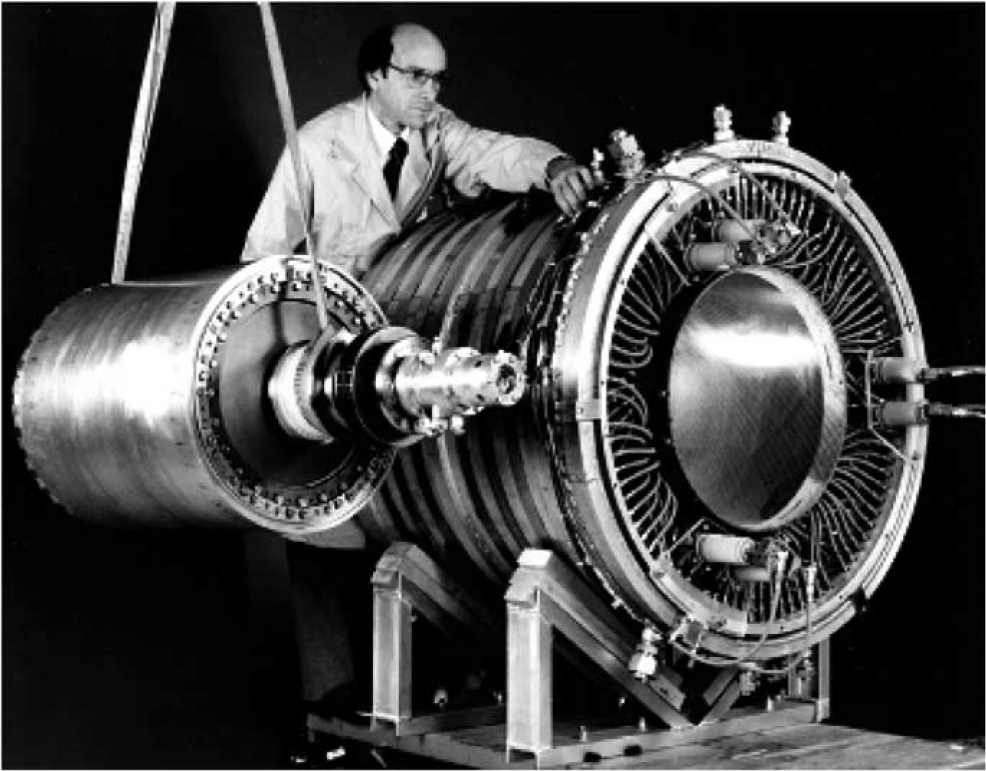
\includegraphics[width=0.3\textwidth]{GE_LTS_machine}
    \caption{General Electric's 20 MW low-temperature superconducting generator with Nb-Ti wire (1981) \cite{Barnes2005}.} 
    \label{GE_LTS_machine}
  \end{figure}

  \begin{figure}[]
    \centering
    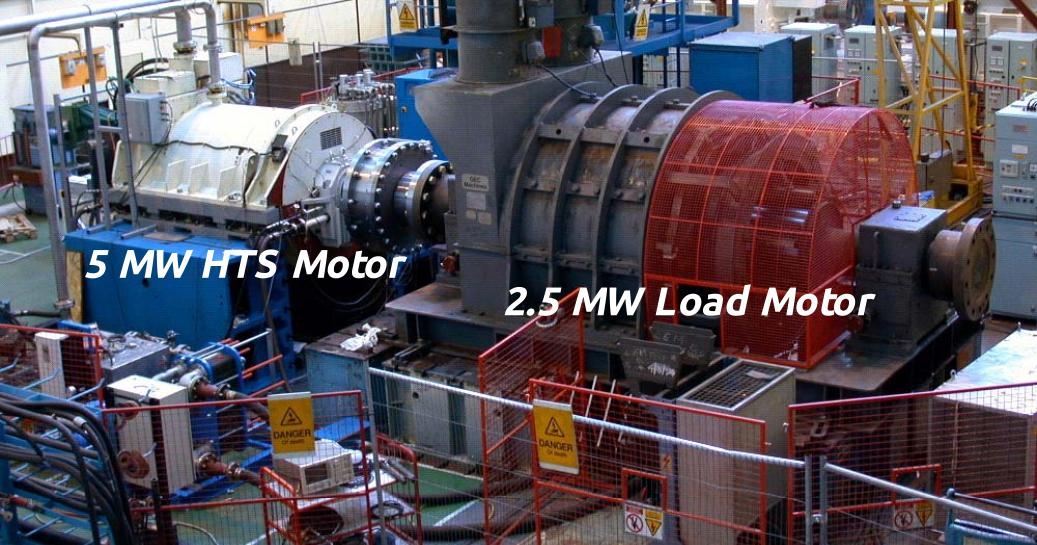
\includegraphics[width=0.45\textwidth]{converteam_5MW}
    \caption{Converteam 5 MW HTS ship propulsion motor coupled to test machine  \cite{Kalsi2004h}.} 
    \label{converteam_5MW}
  \end{figure}

An alternative application area for superconducting machines is direct-drive power take-off systems for large wind turbines. Average size of onshore wind turbines are limited in 3--3.5~MW range due to transportation restrictions and low wind speeds. However, there is a trend towards larger wind turbines for offshore installations. This trend can be seen in Fig. \ref{offshore-turbine-size}, which shows the average turbine size increased from 2 MW to 6 MW between 2002 and 2012. However, this trend seemed to stuck in the 6 MW range due to limitations of the existing power take-off alternatives. 

Larger wind turbines reduces the installation and maintenance cost per MW, and benefit from higher wind speeds. In \cite{Abrahamsen2010}, it is stated that 10 MW offshore wind turbines are desirable in 2020. This is a ambitious challenge to achieve with the existing power take-off (PTO) systems. The geared systems, which is the most common PTO system, have some reliability issues and the mass of the gearbox increases enormously with increasing torque requirements. Direct-drive permanent magnet generators (DDPMG) also suffer from high mass problem and the diameter of these machines are quite large. 
A mass comparison between conventional direct-drive generators and superconducting machines can be found in \cite{Keysan2011b}. The reduction of the tower head-mass will also help to reduce the cost of installation and structural components costs (e.g. tower, foundation).

\begin{figure}[]
  \centering
  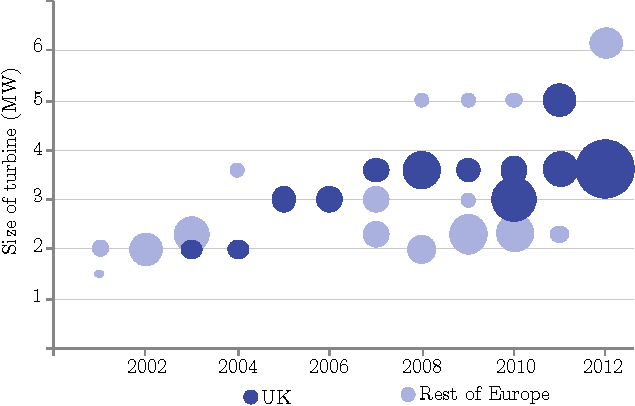
\includegraphics[width=0.45\textwidth]{offshore-turbine-size}
\caption{Commercial offshore wind farms turbine size for UK and Europe. Bubble size is proportional to the wind farm rated output \cite{bvg}.}
  \label{offshore-turbine-size}
\end{figure}


\section{A Review of Superconducting Machines}

The superconducting machines presented in the introduction and many others have the same topology: synchronous machine with a superconducting rotor. Copper windings are usually utilized in the armature, because AC losses in a superconducting coil limits the current density. The stator core can be slotless to eliminate saturation in the stator teeth. Similarly, the rotor can be air-cored or iron-cored. Although, it is possible to achieve higher flux densities with air-cored topologies, they require more superconducting wire.

The synchronous generator with a superconducting rotor introduces many problems. Some of these can be listed as:

\begin{itemize}

  \item \textbf{Rotating Transfer Coupler:} In a rotating superconducting coil configuration, a coupler is required to transfer the coolant from cryocoolers to the rotating frame. This coupler introduces reliability issues and requires regular maintenance. Furthermore, it is the single point of failure for the whole system. There are some designs that aim to simplify or remove the cryocoupler. For example, AMSC plans to put the cold heads in the rotor for their 10 MW, 10 rpm generator design \cite{amsc_presentation}, but the design still requires couplers. General Electric plans to eliminate cryocouplers by using a stationary superconducting coil and a rotating armature configuration \cite{Stautner2012}. However, the design requires high current electrical brushes, which require regular maintenance.

  \item \textbf{Electric Excitation System:} On top of the rotating transfer coupler, brushed or brushless excitation systems are required to excite the superconducting field winding.

  \item \textbf{Torque Transfer Structure:} Electromagnetic torque is generated on the superconducting winding in the conventional superconducting machine topology. Thus, a torque transfer tube is required that extends through cryogenic temperature to room temperature. Usually carbon fibre materials are used to minimize the heat loss, but design of these components are difficult and increases the cost.

  \item \textbf{Transient forces in SC coil:} In a rotating superconducting winding, superconducting tape is exposed to centrifugal and other transient forces. Second generation HTS tapes are in crystal structure and are prone to high stresses and bending. Any cracks or deformations in the superconducting coil can trigger a quench.
\end{itemize}

\vspace{0.5pc}

Other types of superconducting machines are also proposed in the literature. Instead of a superconducting field winding, magnetised bulk superconducting materials can be used, which is similar to a permanent magnet generator. Bulk superconductors can be magnetized in situ or externally. External magnetization is not a feasible method for large scale applications since it would be extremely difficult to handle the pre-magnetized bulk superconductors during the machine assembly. Moreover, if the cooling system fails,  the superconducting magnets will de-magnetize and the machine will be required to be disassembled.  
Thus, in situ magnetization method is the only feasible method for superconducting machines. 
In \cite{Matsuzaki2007}, HTS bulk magnets are magnetized by the pulsed field magnetization method by using a pair of the armature coils. However, the maximum flux density magnitude is limited by the current density of armature coils. There are some novel flux pumping methods that magnetize superconductors gradually by magnetic flux or thermal waves such as \cite{Masson2007b,Coombs2009}. Although these methods have some great potential, they are not proven for large scale applications yet.

There are also a few fully superconducting machine designs, but AC losses in the superconducting coils limit the operation frequency of such machines. A 10 MW, 10 rpm fully superconducting machine is presented in \cite{Terao2012}, but it requires 250--300~km of HTS tape and MgB2 wire each, which makes the design economically infeasible. Advanced Magnet Lab is also investigating a 10~MW, 10~rpm fully superconducting generator, which is expected to be manufactured in 2015. A double-helix superconducting winding configuration is proposed to minimize the AC loses on the armature coils and to limit the flux penetrating into the coils. Weight, including the cooling system, is expected to be 70 tonnes \cite{Masson2011}.

\section{Requirements of a Wind Turbine Generator}

There are many direct-drive superconducting generator designs for large offshore wind turbines, most of which are 10~MW, 10~rpm generators. Although, designers usually concentrate on the electromagnetic optimization, and performance of the machine, they usually neglect the harsh operating conditions and extra requirements of an offshore wind turbine. These can be listed as follows:

\begin{itemize}
  \item \textbf{Reliability:} The maintenance of offshore wind turbines are very difficult and expensive. Furthermore, access to turbine is subject to the weather and the sea conditions, which add weeks or even months of lost electricity generation income on top of the repair cost. Thus, the reliability of an offshore wind turbine is very critical. The reliability of superconducting machines is questionable, but it can be improved by minimising extra equipments and moving parts (such as cryocouplers or electric brushes). 

  \item \textbf{Redundancy:} There are some subsystems that can not be eliminated in a superconducting machine, such as the refrigeration system. In this case, redundancy is essential, in a way that any failures should not cause down times until the next planned maintenance, which can be once in a year.

  \item \textbf{Modularity:} Modularity is another form of redundancy. Modularity has two advantages: firstly, even if a section of the PTO system fails the remaining sections can operate at partial load. For example, Clipper Wind developed a wind turbine (C93 Liberty) that has four parallel PM generators coupled to the gearbox. Thus, a failure in one of the generators will only result in 25 \% loss in the power output. Secondly, by modularity each section will be kept in manageable sizes, and can be replaced by on-site cranes without the need for expensive crane vessels. It is stated in \cite{Kaiser2007} that the replacing a gearbox (of an onshore wind turbine) can cost as much as 10 \% of the initial construction cost. It is a much difficult and expensive task to replace gearbox or drive-drive generator for an offshore wind turbine.

  \item \textbf{Tower Head Mass:} A lower tower head mass help to reduce the installation cost and manufacturing cost by reducing the structural mass requirements of the turbine. The tower head mass becomes much more important in far offshore floating wind turbines. In the design of superconducting machines, the active material mass is usually optimised, but the structural mass is neglected. However, due to increased airgap flux densities, the Maxwell stress acting on the generator structure is higher and a heavier structure may be required. Thus, the optimisation of the structural mass is very important in the superconducting machine design.

  \item \textbf{Cost:} The cost of the power take-off system for a wind turbine is also very critical, and the cost of a superconducting machine is usually dominated by the cost of superconducting tape. In the common designs, the superconducting tape requirement is usually in the order of hundreds of kilometres. Thus, MgB2 wires becomes a favourable option even if its critical temperature is lower. General Electric, plans to use NbTi wires (operating temperature 6 K), to further reduce the cost of the wire \cite{fair2012}.


 \end{itemize}

\section{Proposed Generator} % (fold)
\label{sec:proposed_generator}

A transverse flux superconducting machine topology was proposed in \cite{Keysan2011e,Keysan2012a} (see Fig. \ref{rotational_claw_schematic}). The generator consists of a single loop-shaped stationary superconducting coil, a modular rotor that consists of claw-poles made of laminated steel. The biggest advantage of the design is having a stationary superconducting coil and armature. The only rotating part in the machine is modular claw pole structure. However, the initial design has unbalanced forces acting on the claw pole rotor and also requires use of soft magnetic composite (SMC) material in the inner stator. Thus, it is not really suitable for a large scale applications.

\begin{figure}[]
  \centering
  \subfloat[Side view.]{\label{rotational_claw_side}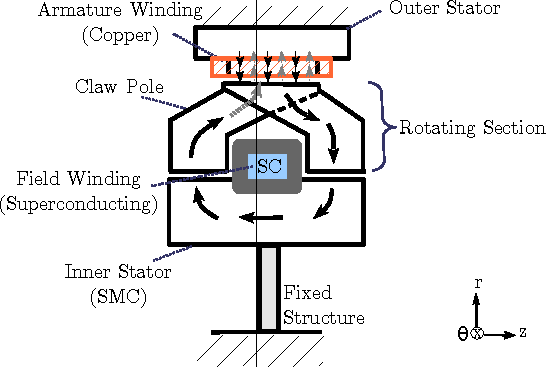
\includegraphics[scale=0.7]{rotational_claw_schematic}}

  \subfloat[Front section view.]{\label{rotational_claw_front}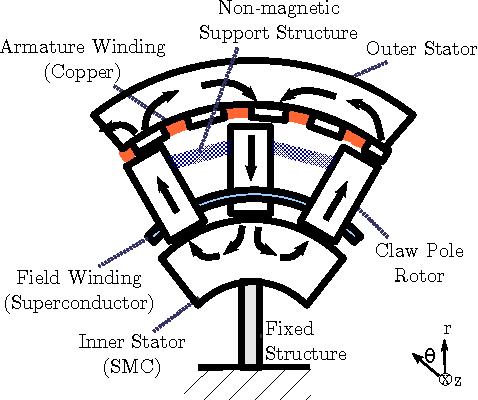
\includegraphics[scale=0.7]{rotational_claw_schematic2}}
    \caption{Basic schematic and flux lines in the transverse flux claw pole superconducting machine \cite{Keysan2011e}.} 
    \label{rotational_claw_schematic}
\end{figure}

The machine presented in Fig. \ref{rotational_claw_side} can be rotated 90 degrees to obtain an axial flux machine as shown in Fig. \ref{axial_claw_pole}. Then, two axial machine claw poles machines can be combined to obtain a double-sided machine as shown in Fig. \ref{double_claw_pole}. In this configuration, there is also a single superconducting field winding, but the design has two independent armature windings. The magnetic flux travels along the claw poles and links the independent armature windings on each end. The magnetic attraction forces acting on the claw pole are symmetrical and cancel each other (assuming the air-gap clearances on each side are equal). 

In the double-claw machine, soft-magnetic composite material is no longer needed as the flux through the field core travels only in the axial direction, and the field core can be manufactured from steel laminations.
The advantages of the double-sided claw pole topology can be summarised as:

\begin{itemize}
  \item Stationary superconducting field winding (no transfer couplers).
  \item No electromagnetic forces acting on the superconducting coil (simpler mechanical support).
  \item Magnetic attraction forces on the claw poles are symmetrical and cancel each other (reduced structural mass).
  \item Two independent armature windings (modularity).
\end{itemize}

\vspace{0.5pc}

\begin{figure}[]
  \centering
  \subfloat[Axial claw pole.]{\label{axial_claw_pole}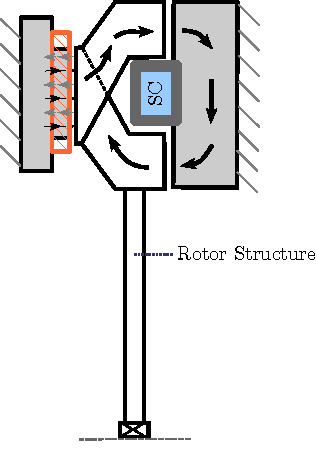
\includegraphics[scale=0.66]{axial_claw_pole}}
  \subfloat[Double-sided claw pole.]{\label{double_claw_pole}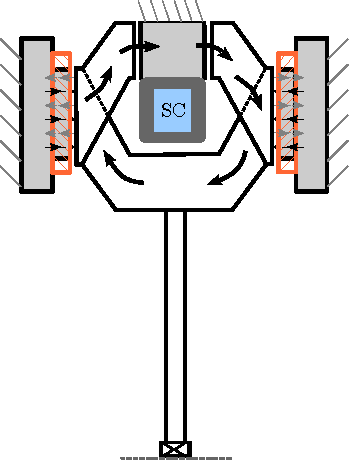
\includegraphics[scale=0.7]{double_claw_pole}}
    \caption{Evolution of the double sided transverse flux claw pole topology.} 
    \label{claw_pole_evolution}
\end{figure}

The topology is simulated using a 3D FEA software. The full model and the model with pole symmetry is presented in Fig. \ref{double_claw_parts}. In the model a single field winding is used. The magnetic flux vectors in the claw pole are shown in Fig. \ref{double_claw_B_vector_front}. It can be seen that the claw pole is saturated up to 2.3 T. In order to achieve such a high flux density, Vacuumschmelze's VacoFlux50 has been used. VacoFlux50 is a cobalt-iron alloy which can be manufactured in laminations and has an impressive magnetic saturation limit with 2.35 T at 16 kA/m \cite{vacoflux}. The magnetisation direction in the claw poles remains same regardless of the rotation. Thus, it is expected to have low core loss in these highly saturated areas.

The flux density magnitude in the stator teeth at mid-coil radius is plotted in Fig. \ref{tooth_flux}. The graphs show that the flux density in the stator teeth can reach up to 2.1 T.

\begin{figure}[]
  \centering
  \subfloat[Section of the machine.]{\label{double_claw_parts_iso}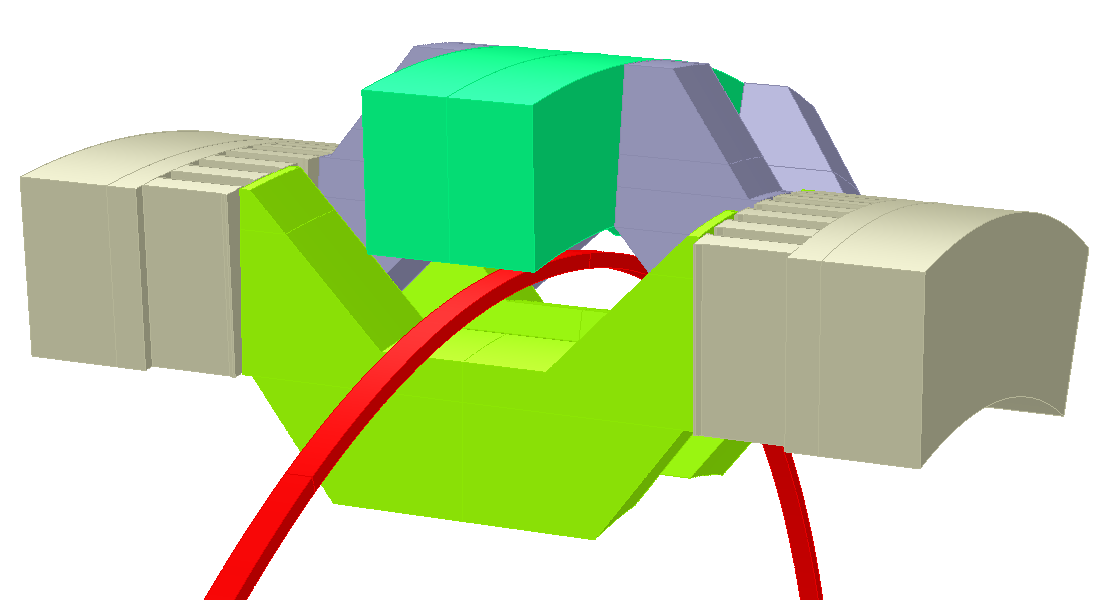
\includegraphics[width=0.45\textwidth]{double_claw_parts_iso}}

\subfloat[Isometric view.]{\label{double_claw_full}   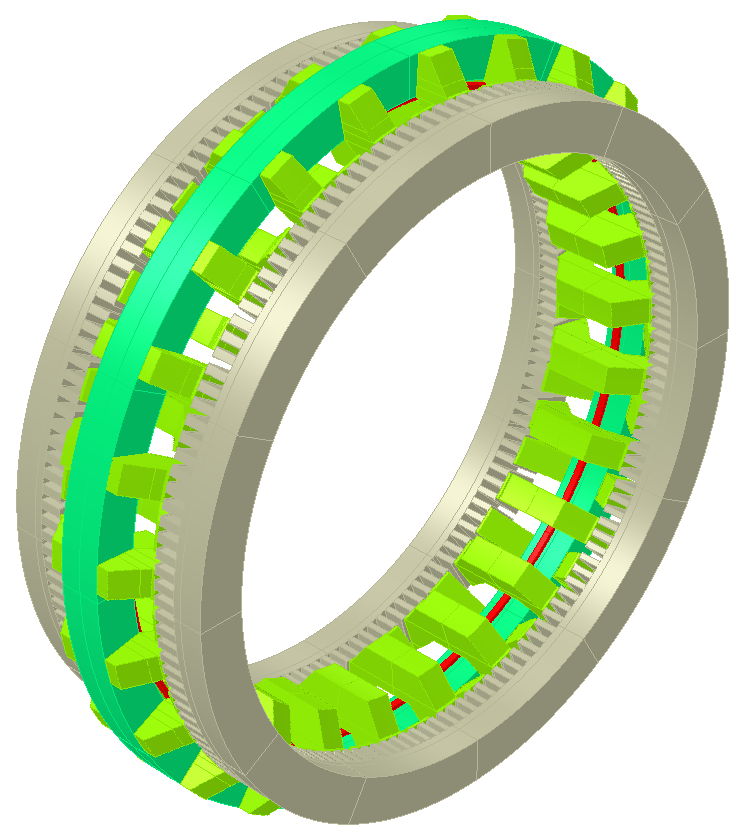
\includegraphics[]{double_claw_full}}

 \caption{The double-claw pole machine FEA model.} 
 \label{double_claw_parts}

\end{figure}


\begin{figure}[]
\centering
 \subfloat[Flux density vectors (The vector size is proportional to the flux density magnitude).]{\label{double_claw_B_vector_front}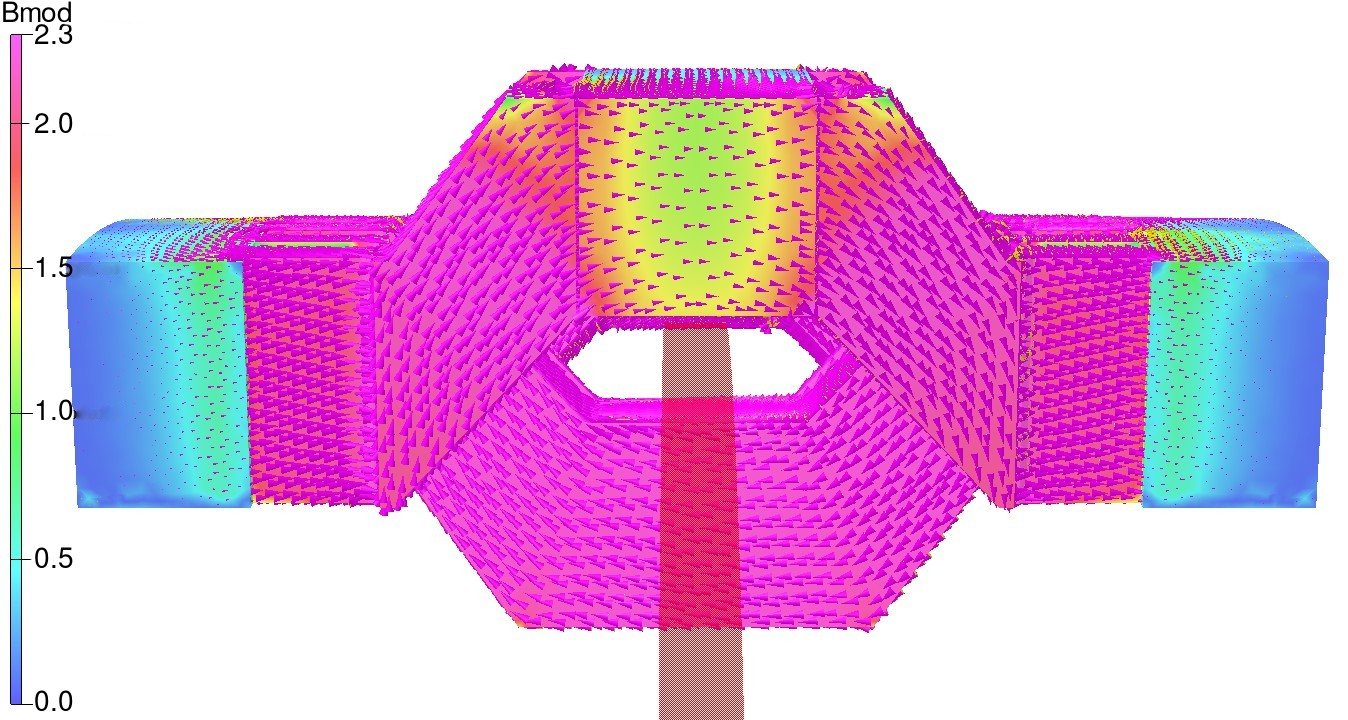
\includegraphics[width=0.45\textwidth]{double_claw_B_vector_front}}

\subfloat[Flux density magnitude distribution in the stator teeth (mid-coil radius) ($N_{slot}=192$).]{\label{tooth_flux}
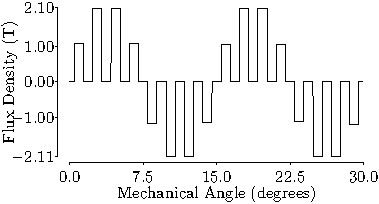
\includegraphics[]{stator_Bz_Nslot_192}}
  \caption{FEA simulation results for the double claw-pole machine.} 
  \label{FEA_results}
\end{figure}


\section{Modular Cryostat} % (fold)
\label{sec:modular_cryostat}

The double-claw pole machine is designed for large diameter, high torque applications, but a single loop shaped superconducting coil (see Fig. \ref{double_claw_parts}) can cause some problems in manufacturing and transportation. Also, the machine needs to be disassembled to replace the superconducting coil.

In the original design, the superconducting coil and the cryostat are fixed to the inner surface of the field core as shown in Fig. \ref{single_cryostat}. Assume that another coil is mounted on the outer surface of the field core as in \ref{double_cryostat}, which conducts current in the opposite direction. Now, assume that the cryostat and the field core are divided into two sections as shown in \ref{sectioned_cryostat}, which results in two independent cryostats. It is also possible to use more than two cryostat sections in a large diameter machine.

In this configuration, it is possible to manufacture and transport each core section separately. Furthermore, even if one of the cryostats fails, the machine can still operate at partial load until the next maintenance. It is also much easier to replace the failed cryostat. 

\begin{figure}[]
  \centering
  \subfloat[Single cryostat.]{\label{single_cryostat}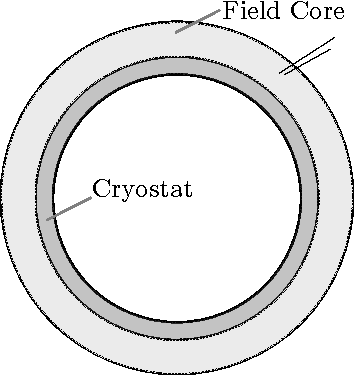
\includegraphics[scale=0.65]{single_cryostat}}  \hfill
  \subfloat[Double cryostat.]{\label{double_cryostat}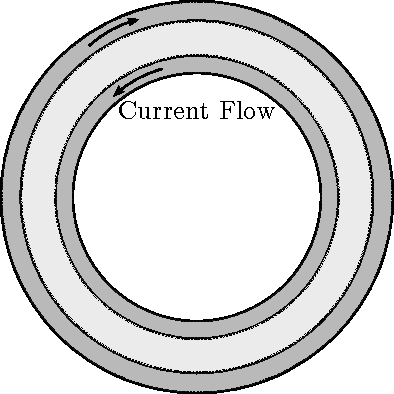
\includegraphics[scale=0.6]{double_cryostat}} \hfill 
  \subfloat[Sectioned cryostats.]{\label{sectioned_cryostat}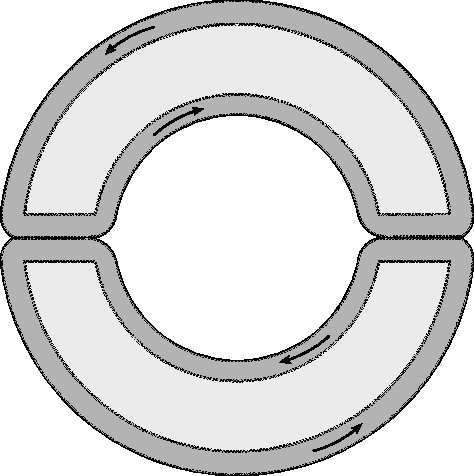
\includegraphics[scale=0.5]{sectioned_cryostat}}
    \caption{Different cryostat designs for the double-claw pole machine. Front view.} 
    \label{cryostat_variants}
\end{figure}


% section modular_cryostat (end)

\section{Conclusion} % (fold)
\label{sec:conclusion}

Operating conditions and requirements of an offshore wind turbine generator are different from a superconducting machine installed in a controlled environment. The authors believe existing superconducting generator designs with a rotating superconducting field winding have many shortcomings in terms of reliability and modularity. Any serious faults in these machine results in a turbine shut-down and require disassembly of the generator, which is very expensive for offshore wind turbines.

In this paper, the transverse flux machine presented in \cite{Keysan2011e} has been improved by introducing the double-claw pole concept. In this concept, the machine has two independent armature windings. The modularity is further improved by the sectioned cryostat concept. Sectioned cryostats introduces modularity and redundancy to the system. If a fault occurs in one of the cryostats the remaining ones can still generate electricity at partial load. Furthermore, the cryostats can be removed and replaced using small on-site cranes without dissembling the machine.

FEA simulations of the generator design showed that flux densities up to 2.1 T are achieved in the stator teeth, which will help to increase the power density. The magnetic attraction forces between rotor and stator are symmetrical. Thus, the structural mass of the generator is expected to be high, compared to other designs. Design and optimization of a 10 MW, 10 rpm generator is still ongoing and will be presented in future.




% section conclusion (end)

% \section*{Acknowledgements}

% The acknowledgement for funding organisations etc. should be placed in a
% separate section at the end of the text.

% Thank you for your cooperation in complying with these instructions.
%\newpage

\bibliography{pemd-2014}

\bibliographystyle{ieeetr}

% \begin{thebibliography}{9}
% \vspace{1pc}

% \bibitem{}A. B. Author, C. D. Author. ``Title of the article'',
% \textit{The Journal}, \textbf{volume}, pp.~110--120, (2000).\vspace{.4pc}
% \end{thebibliography}


\end{document}
